\documentclass[a4paper]{article}

\usepackage[english]{babel}
\usepackage[utf8]{inputenc}
\usepackage{amsmath}
\usepackage{graphicx}
\usepackage[colorinlistoftodos]{todonotes}

\title{Analice User Guide}

\begin{document}

\maketitle
\tableofcontents

\newpage

\section{Introduction}
Hello and welcome to Analice. This tool is used to perform your analyses for you so that you can get answers from data you collected. This manual will guide you through the process of using this program.

\section{The Main Program}
After the main program has been launched you will get the window as seen in figure~\ref{fig:main}. There are 4 tabs through where you can navigate. The tabs are:

\begin{figure}[h]
	\centering
	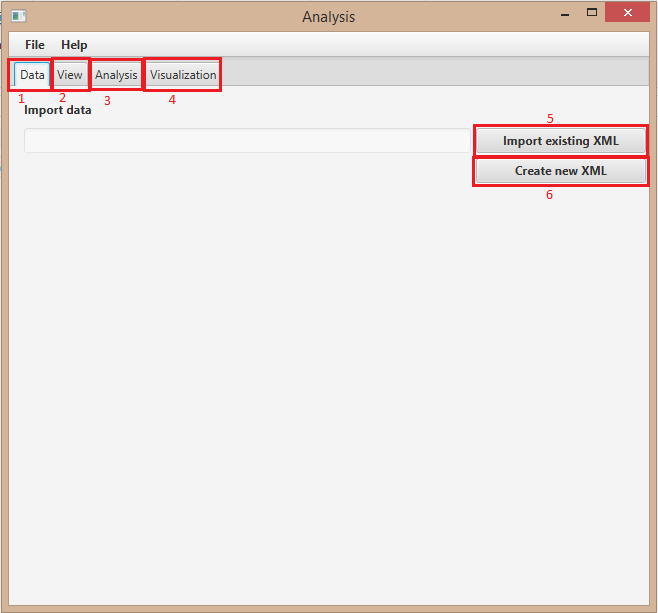
\includegraphics[scale=0.6]{mainprogram.png}
	\caption{}
	\label{fig:main}
\end{figure}

\begin{enumerate}
\item The data tab (1) which is currently showing. In this tab you can import data from the system. 
\item The view tab (2) . In this tab you can view the data which is currently loaded into the program.
\item The analysis tab (3). In this tab there is a simple text editor in which you can write SUGAR scripts to perform analyses.
\item The visualization tab (4). In this tab you can create, view and export different visualizations.
\end{enumerate}

\section{Importing data}
The first step to create an analysis is getting the data which we work with into the system. The raw data that our program supports must be saved in either a delimited plain text file or an excelfile. For future reference we will call these files datafiles. The whole process of inputting data is done by specifying datafiles in an XML file. There are 2 different ways to import this data. It can be done by creating a new XML file using the XML wizard, or by importing an existing XML file.

\section{XML wizard}
We can select files and specify its properties using the XML wizard. The basic approach to create a new XML file is by pressing the "Create new XML" (figure~\ref{fig:main} (5)) button in the data tab. Next the window will appear as in figure~\ref{fig:xmlwizard}.

\begin{figure}[h]
	\centering
	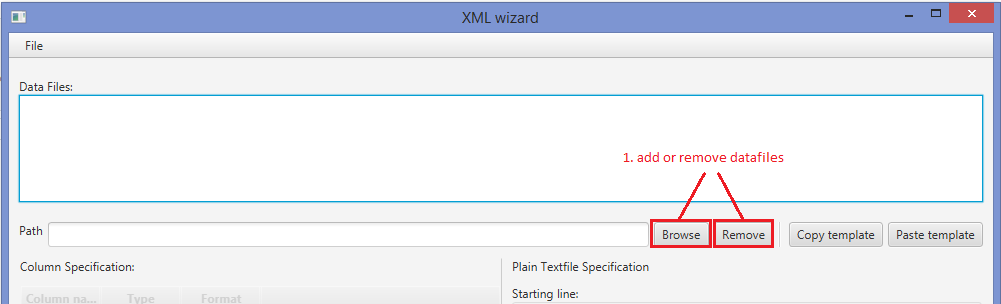
\includegraphics[scale=0.5]{xmlwizard.png}
 	\caption{The XML wizard}
	\label{fig:xmlwizard}
\end{figure}

To begin the specification we can follow these steps:

\begin{figure}[h]
	\centering
	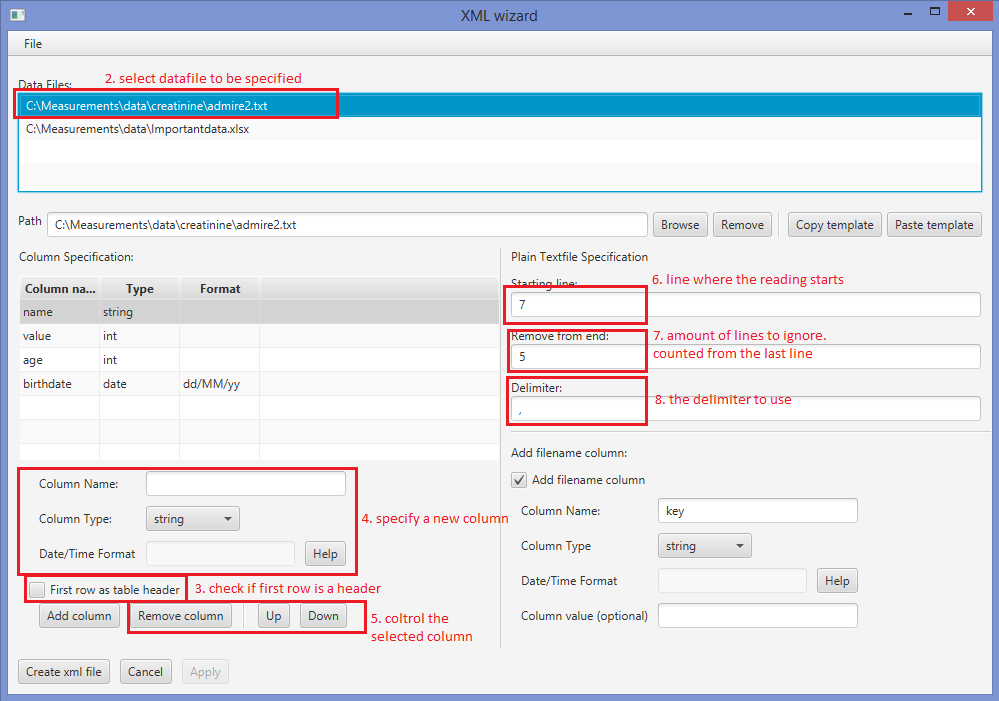
\includegraphics[scale=0.5]{xmlwizardfilled.png}
 	\caption{Filling in the XML wizard}
	\label{fig:xmlwizardfilled}
\end{figure}

\begin{enumerate}
\item Add new datafiles specifications. For each file you want to specify, press the "Browse" button to select a datafile from the system. You can remove an unwanted datafile by selecting the datafile and then press the "Remove" button.
\item For each datafile to be specified, select the datafile in the list and continue following the next steps.
Next we want to specify the columns of the file. 
\item If the file contains a first row that functions as a header, check the "First row as table header" checkbox so the no names have to be given to columns. 
\item To specify a new column, fill in the properties of the column and press the "Add column" button. Do this for each column in the datafile. The columns in the datafile must be in the same order as specified in the column specification. If the type of the column is a temporal value, it is necessary to specify a format for the date before adding the column specification.
\item If you make a mistake and want to change order of columns, the "Up" and "Down" buttons can be used to control the selected column specification and the "Remove" button removes the selected column specification.

The next three steps are only necessary for specifying a plain text file. These are in the "Plain Textfile Specification" area.
\item Starting line: The starting line of the file is the line at which the first column of significant data starts. So if the plain textfile contains a header, this can be skipped by specifying the starting line.
\item Remove from end: This is the amount of lines NOT to read as data counted from the end of the plain textfile. This can for example be a footer.
\item The last thing we need to specify is the delimiter of the file. The columns in the plain textfile must be split by some character. This character must be specified here. These can for example be a comma (,) or a tab character ($\backslash$t) etcetera.
\\\\

OPTIONAL: Specifying a filename column. In the "Add filename column" area you can choose if you want to add a column to the selected datafile specification. This column must have a name so you can reference to this in future analyses. The type of this column must also be specified (same here: if the type is a temporal value, the format must be specified). All the values of this column will be filled with the same value, namely the name of the file without the extension. This column can be used later to specify a connection between different tables based on this key value. It is also possible to specify your own value for this column instead, by filling in the "Column value" field. Don't forget to apply your changes after modifying these settings for a datafile.
\\\\

Tip: If you have multiple files with the same specification, you can copy a template of this file by selecting the file and pressing the "Copy template" button. After this is done you can apply the copied specification by selecting the target datafile and pressing the "Paste template" button.
\\\\

After all the specifications are correctly set we can create the XML file. Choose the path to save the XML file and after that the wizard will close and the program will start loading the datafiles.

It is also possible to edit a previously created XML file using the XML wizard. This is done in the wizard by going to File -> Load and then choose the XML file.

\end{enumerate}

\section{Existing XML files}
We can also use an existing xml file (if you created one earlier). You can import the specified datafiles immedeately by using the "Import existing XML" button in the data tab. After you choose the XML file, the specified datafiles will be imported into the program.

\newpage

\section{View data}
\begin{figure}[h]
	\centering
	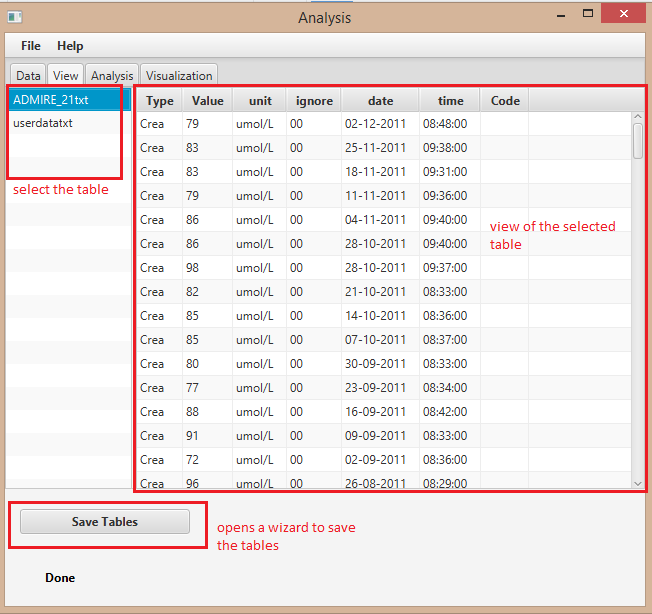
\includegraphics[scale=0.5]{viewtab.png}
 	\caption{The view tab}
	\label{fig:viewtab}
\end{figure}
To see the data that has been imported into the program you can switch to the view tab. Here you can see a table which contains this data. To see a different table you can just change the selection and the view will change.

It is also possible to save the tables by pressing the "Save Tables" button. This will open the wizard as seen in figure~\ref{fig:savetables}

\begin{figure}[h]
	\centering
	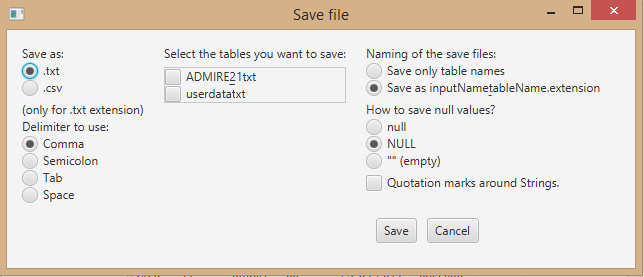
\includegraphics[scale=0.5]{savetables.png}
 	\caption{The save tables wizard}
	\label{fig:savetables}
\end{figure}

\newpage

\section{Analysis}
In the analysis tab you can perform an analysis. For creating the analysis we refer you to the \textit{language specification} document. The analysis can be performed after the script has been entered into the by pressing the "execute" button. After the analysis is completed, results will be automatically processed into the view.
\begin{figure}[h]
	\centering
	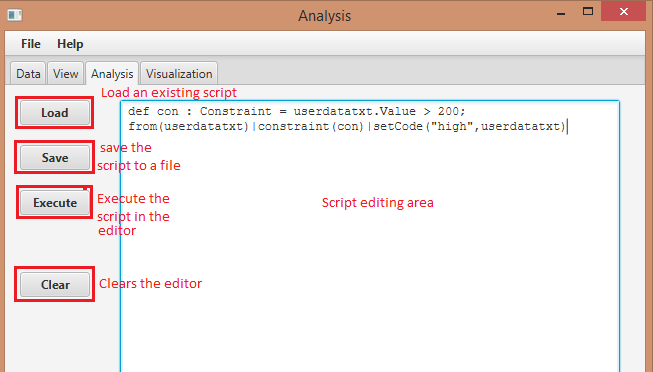
\includegraphics[scale=0.5]{analysistab.png}
 	\caption{The analysis tab}
	\label{fig:analysistab}
\end{figure}

\newpage

\section{Visualizations}
In the visualization tab you can create a visualization. Visualizations can only be made when there is already data present in the program. To make a state transition matrix the table must contain codes first. The codes can be added using analysis scripts.
\begin{figure}[h]
	\centering
	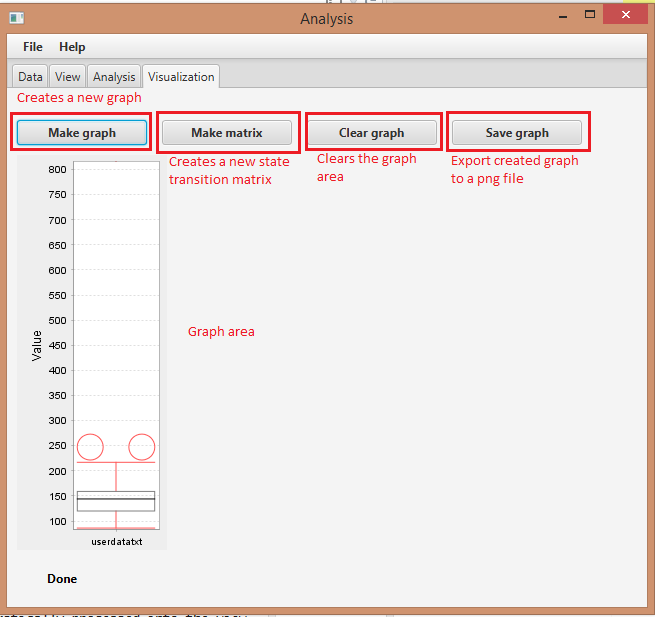
\includegraphics[scale=0.5]{visualizationtab.png}
 	\caption{The visualization tab}
	\label{fig:visualizationtab}
\end{figure}



\end{document}